\documentclass[a4paper, 12pt]{article}%тип документа

%отступы
\usepackage[left=2cm,right=2cm,top=2cm,bottom=3cm,bindingoffset=0cm]{geometry}

%Русский язык
\usepackage[T2A]{fontenc} %кодировка
\usepackage[utf8]{inputenc} %кодировка исходного кода
\usepackage[english,russian]{babel} %локализация и переносы

%Вставка картинок
\usepackage{wrapfig}
\usepackage{graphicx}
\graphicspath{{pictures/}}
\DeclareGraphicsExtensions{.pdf,.png,.jpg}

%оглавление
\usepackage{titlesec}
\titlespacing{\chapter}{0pt}{-30pt}{12pt}
\titlespacing{\section}{\parindent}{5mm}{5mm}
\titlespacing{\subsection}{\parindent}{5mm}{5mm}
\usepackage{setspace}

%Графики
\usepackage{multirow}
\usepackage{pgfplots}
\pgfplotsset{compat=1.9}

%Математика
\usepackage{amsmath, amsfonts, amssymb, amsthm, mathtools}

\begin{document}

\begin{titlepage}

\begin{center}
%\vspace*{1cm}
\large\textbf{Московский Физико-Технический Институт}\\
\large\textbf{(государственный университет)}
\vfill
\line(1,0){430}\\[1mm]
\huge\textbf{Вынужденные колебания в электрическом контуре}\\
\line(1,0){430}\\[1mm]
\vfill
\large Сибгатуллин Булат, ФРКТ\\
\end{center}

\end{titlepage}

\section*{Цель работы}
	Исследование вынужденных колебаний и процессов их установления.
	\section*{Оборудование}
	Генератор звуковой частоты (ЗГ), осциллограф (ЭО), вольтметр, частотометр, ёмкость, индуктивность, магазин сопротивлений, универсальный мост.
	\section*{Экспериментальная установка}
	\begin{figure}[h!]
		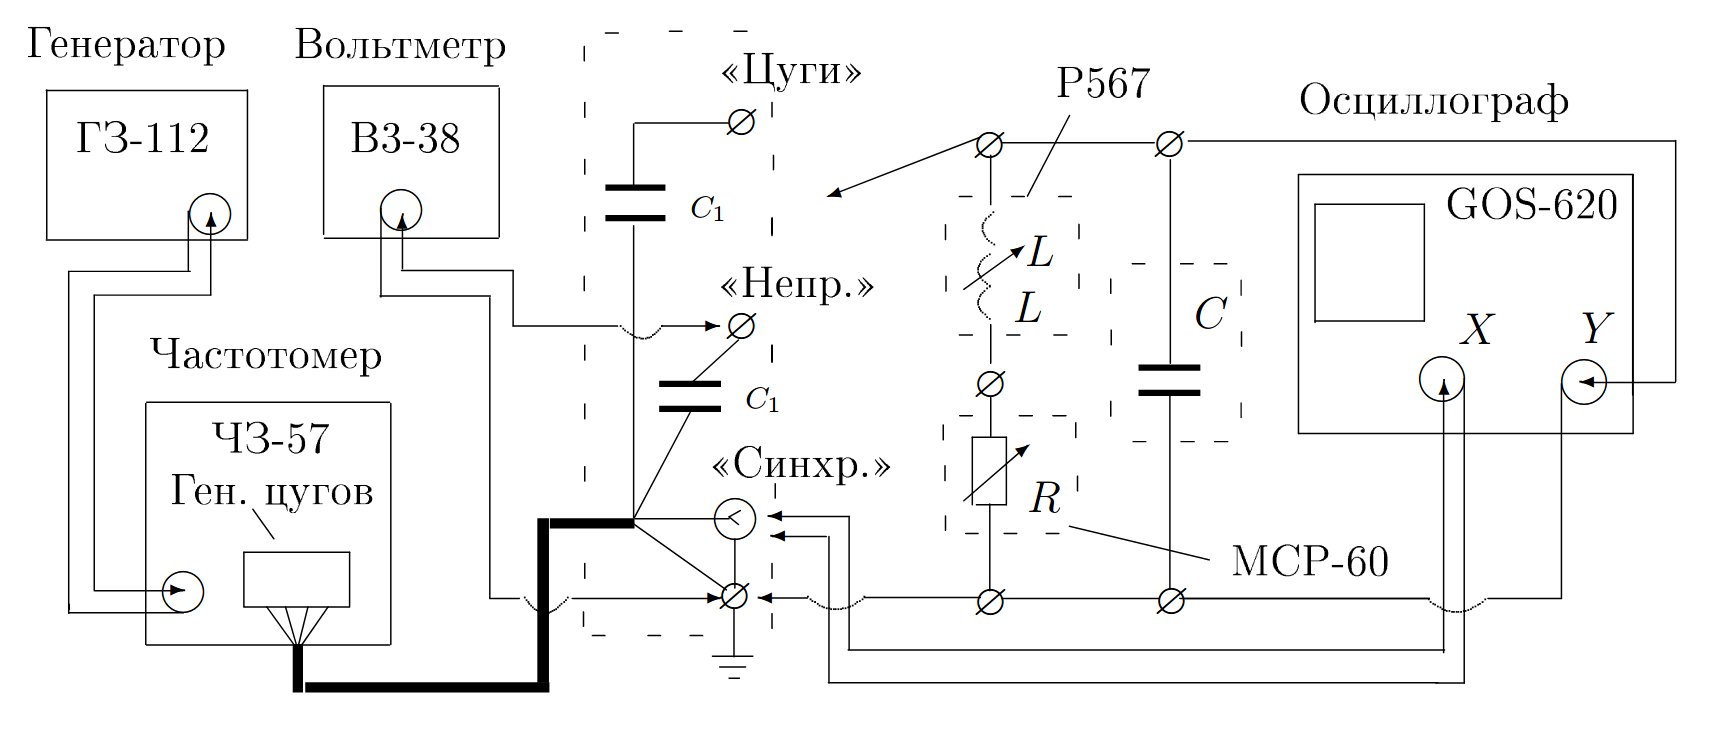
\includegraphics[width = 1.0\linewidth]{ust.png}
	\caption{Схема установки для исследования вынуждённых колебаний}
	\end{figure}
	\section*{Теоретическая часть}
	Для экспериментального исследования резонансной кривой тока в последовательном колебательном контуре можно снять зависимость амплитуды напряжения на резситоре $R$ от частоты генератора (при постоянной амплитуде выходного напряжения генератора). Но импеданс этого контура включает в себя выходной импеданс генератора. Мы должны быть уверены, что выходной импеданс генератора много меньше импеданса контура и не влияет на процессы, происходящие в этом контуре.
	
	Для устранения этого влияния можно использовать схему, представленную на рисунке (1): синусоидальный синал с генератора подаётся на параллельный колебательный контур через небольшую разделительную ёмкость $C_1$. Напряжение с ёмкости кнтура $C$ поступает на вертикальный вход ЭО.
	
	Зависимость амплитуды этого напряжения от частоты генератора будет практически совпадать с резонансной кривой для последовательного контура, если импедансы возбуждающей и измеряющей цепей (сопротивления переменному току) намного превосходят импеданс самого контура вблизи резонанса $Z_\text{рез} \approx L / (RC) = Q / (\Omega C)$. Разделительная ёмкость $C_1$ выбирается настолько малой, что в рабочем диапазоне частот её импеданс $Z_{C_1} = 1/(\Omega C_1)$ много меньше импеданса контура, поэтому в цепи генератора течёт ток практически с постоянной амплитудой, а колебательный контур выполняет роль нагрузочного сопротивления, которое, в свою очередь, зависит от частоты. Поскольку в резонансе сопротивление $Z_\text{рез}$ параллельного контура максимально, то и напряжение на ёмкости $C$ (неизменный ток, умноженный на максимальное сопротивление) тоже максимально. Входное сопротивление осциллографа (измеряющей цепи) достаточно велико: $R_\text{ЭО} \approx 1 \text{МОм}$.
	
	Таким образом, при выполнении условий
	\[
		Z_{C_1} = \frac{1}{\Omega C_1} \gg |Z| = \frac{Q}{\Omega C}, \quad R_\text{ЭО} \gg \frac{Q}{\Omega C}
	\]
	и при условии, что действительная часть импеданса катушки много меньше её мнимой части, резонансная кривая в нашем контуре бует выглядеть так же, как в последовательном: максимум амплитуды при резонансе. Ширина резонансной кривой определяет важную характеристику контура --- добротность.
	
	Добротность контура может быть определена и другими способами, например, по скорости нарастания амплитуды вынужденных колебаний при резонансе или по скорости затухания свободных колебаний. Нарастание и затухание колебаний можно наблюдать на экране осциллографа, если на контур подаются цуги --- отрезки синусоиды, разделённые интервалами, в течение которых сигнал отсутствует. Чем выше добротность, тем медленне нарастают и медленнее затухают колебания в контуре. Количественные оценки можно сделать, сли определить логарифмический декремент затухания по скорости нарастания или затухания колебаний. В условиях резонанса огибающая затухающих колебаний это перевёрнутая огибающая нарастающего участка, поэтому при расчёте логарифмического декремента по затуханию нет необходимости использовать амплитуду установившихся колебаний $U_0$, которая в контуре с высокой добротностью иногда не успевает установиться за время продолжительности цуга.
	
\section{Ход работы}

\begin{enumerate}

\item Найдем частоту резонанса - $\nu_0 = 1550 \: \textit{Гц}$. Меняя частоту генератора в обе стороны снимем зависимость показаний амперметра и вольтметра от частоты сигнала. Проведем аналогичные измерения для другого значения $R$, данные запишем в таблицу.

\begin{figure}[h!]
    \begin{center}
        \begin{minipage}[h!]{0.4\linewidth}          
            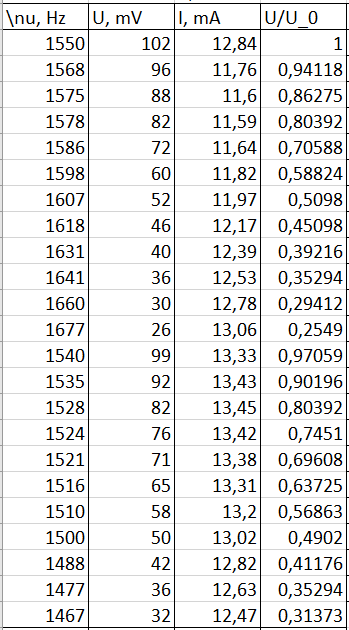
\includegraphics[scale=1]{table1.png}
            \caption{R = 0 Ом}
            \label{fig:Image1}
        \end{minipage} 
        \hfill
        \begin{minipage}[h!]{0.4\linewidth}          
            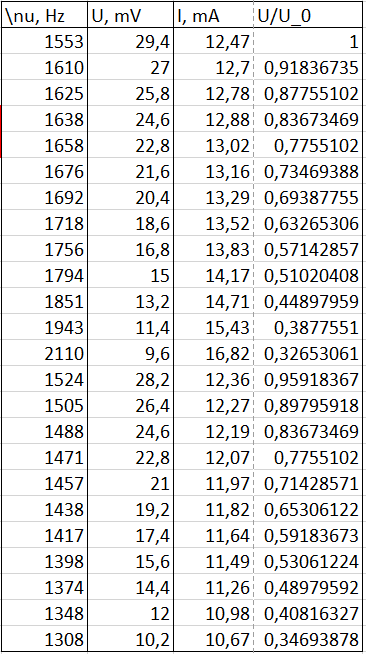
\includegraphics[scale=1]{table2.png}
            \caption{R = 100 Ом}
            \label{fig:Image1}
        \end{minipage}
    \end{center}
\end{figure}

Построим график в координатах $U/U_m = f(\nu / \nu_m)$, где $U_m$ - напряжение на резонансной частоте $\nu_m$.

\begin{figure}[h!]
\centering
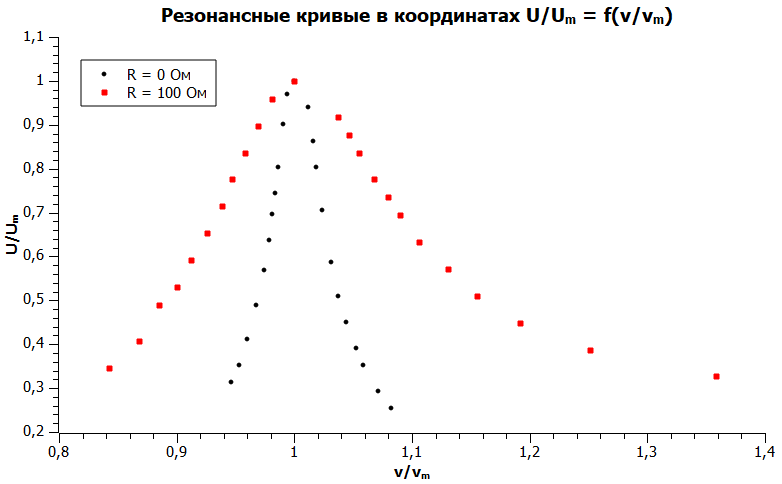
\includegraphics[scale=1]{graph1.png}
\label{fig:Image1}
\end{figure}

\item Рассчитаем добротность по формуле:

\[Q = \frac{\nu_0}{2 \bigtriangleup \nu}\]

\[R = 0: \: Q_0 = \frac{1550}{65} = 23,8\]

\[\sigma_{Q_0} = 0,33\]

\[R = 100: \: Q_{100} = \frac{1550}{235} = 6,59\]

\[\sigma_{Q_{100}} = 0,09\]

\item Рассчитаем добротность контура по скорости нарастания и затухания колебаний. Для этого запишем амплитуды двух колебаний $U_k$ и $U_{k + m}$. Аналогично для затуханий. Запишем данные в таблицу:

\begin{figure}[h!]
\centering
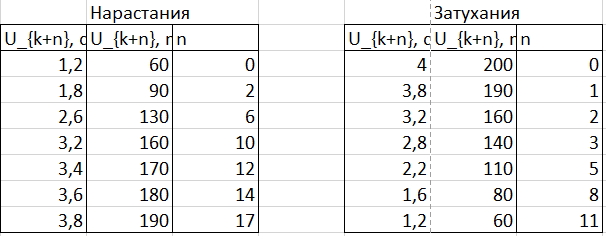
\includegraphics[scale=1]{table3.png}
\caption{R = 0 Ом}
\label{fig:Image1}
\end{figure}

\begin{figure}[h!]
\centering
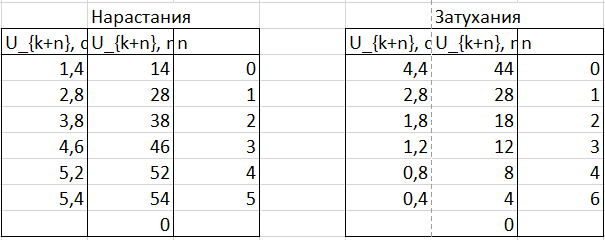
\includegraphics[scale=1]{table4.png}
\caption{R = 100 Ом}
\label{fig:Image1}
\end{figure}

Рассчитаем добротность по формулам:

\[Q_{\text{нар}} = \pi \Big(\frac{1}{n} ln \frac{U_0 - U_k}{U_0 - U_{k+n}}\Big)^{-1}\]

\[Q_{\text{зат}} = \pi \Big(\frac{1}{n} ln \frac{U_k}{U_{k+n}}\Big)^{-1}\]

\[Q_{0\text{нар}} = 28,17 \pm 0,85\]

\[Q_{0\text{зат}} = 33,1 \pm 9,4\]

\[Q_{100\text{нар}} = 1,91 \pm 0,37\]

\[Q_{100\text{зат}} = 2,32 \pm 0,08\]

\item Определим теоретическоее значение добротности контура по формуле:

\[Q = \frac{1}{R}\sqrt{\frac{L}{C}}\]

Запишем параметры установки в таблицу:

\begin{figure}[h!]
\centering
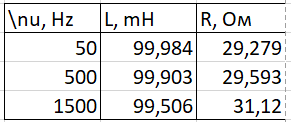
\includegraphics[scale=1]{table5.png}
\label{fig:Image1}
\end{figure}

Определим теоретическое значение добротности контура:

\[Q_0 =  33,2\]

\[Q_{100} = 7,69\]

\item Запишем результаты определения Q в таблицу:

\begin{tabular}{|c|c|c|c|c|c|}
\hline 
R, Ом & $\sum R$  & Кривая & Нарастание & Затухание & Теория \\ 
\hline 
0 & 31,12 &   23,8 & 28,17 & 33,1 & 33,2 \\ 
\hline 
100 & 131,12 & 6,59 & 1,91 & 2,32 & 7,69 \\ 
\hline 
\end{tabular} 

\item Зафиксируем картину биений на экране осциллографа:

\begin{figure}[h!]
\centering
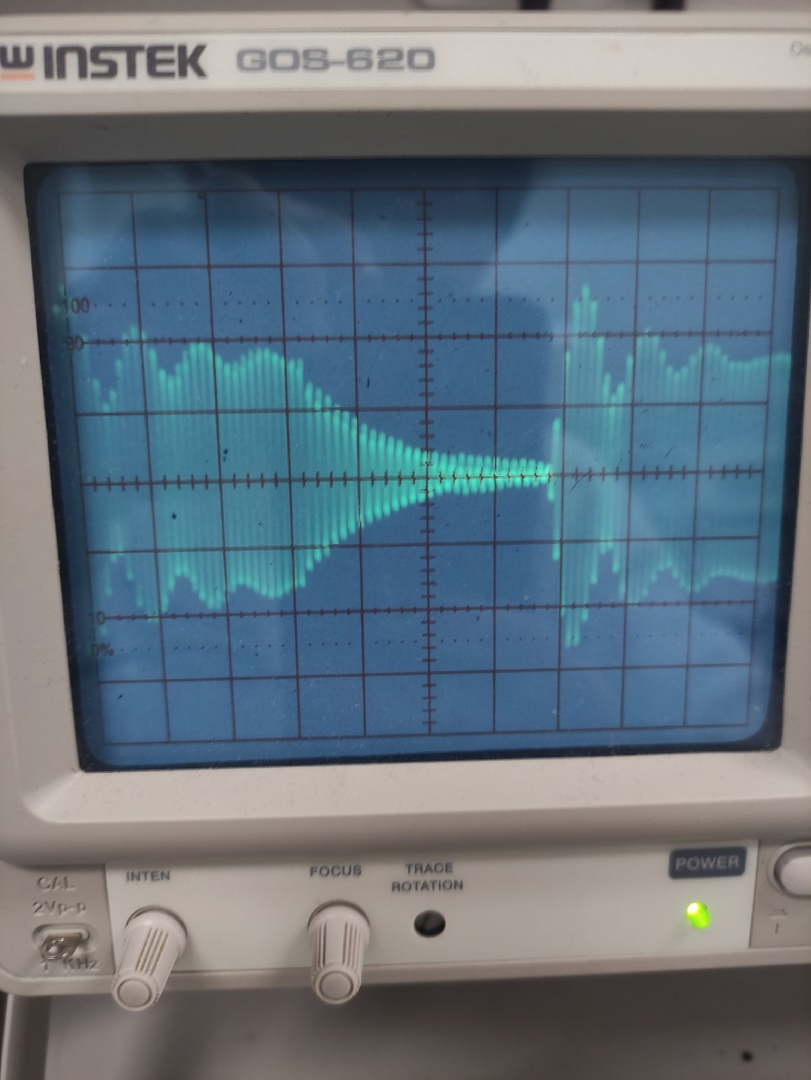
\includegraphics[scale=0.3]{img1.jpg}
\label{fig:Image1}
\end{figure}

\end{enumerate}

\end{document}